% This file was created by matlab2tikz.
%
%The latest updates can be retrieved from
%  http://www.mathworks.com/matlabcentral/fileexchange/22022-matlab2tikz-matlab2tikz
%where you can also make suggestions and rate matlab2tikz.
%
\definecolor{mycolor1}{rgb}{0.00000,0.44700,0.74100}%
%
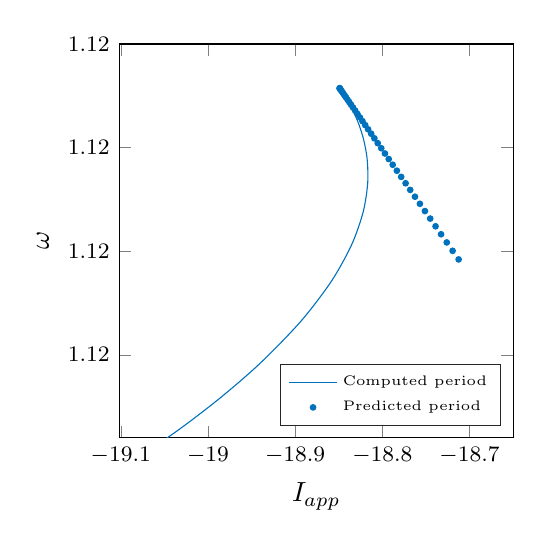
\begin{tikzpicture}[%
mark size=1, baseline
]

\begin{axis}[%
width=5cm,
height=5cm,
at={(0cm,0cm)},
scale only axis,
xmin=-19.1016,
xmax=-18.65,
xlabel={$I_{app}$},
ymin=1.1144,
ymax=1.122,
ylabel={$\omega$},
axis background/.style={fill=white},
every tick label/.append style={font=\footnotesize},
legend style={at={(0.97,0.03)},anchor=south east,legend cell align=left,align=left,draw=white!15!black, font=\tiny}
]
\addplot [color=mycolor1,solid,smooth]
  table[row sep=crcr]{%
-18.8489653934315	1.12114802220414\\
-18.8489569335003	1.12114781667605\\
-18.8489393421973	1.12114738920956\\
-18.8489196326234	1.12114664892115\\
-18.8488660573189	1.1211453463376\\
-18.8487797163129	1.12114324443769\\
-18.8486430782593	1.12113995252602\\
-18.8484360129733	1.12113488564268\\
-18.8481239037578	1.12112721409494\\
-18.8476689345221	1.12111568744199\\
-18.8469884170715	1.12109867773962\\
-18.8460036436019	1.12107368753263\\
-18.8446053073294	1.1210371876481\\
-18.8426415199709	1.1209845386312\\
-18.839961687004	1.12090907812751\\
-18.8364386304914	1.12080187863457\\
-18.8319936885567	1.12065151292485\\
-18.8268134513466	1.12044340712001\\
-18.8215561621181	1.12016094847046\\
-18.8174894589772	1.11978909418206\\
-18.8167852496184	1.11932032311025\\
-18.8219814773802	1.11875974475023\\
-18.835356591212	1.11812066005289\\
-18.8587008410894	1.11741415704896\\
-18.8936385875186	1.11664444632525\\
-18.939628837589	1.11584590767848\\
-18.9831477714225	1.11520733619215\\
-19.0252299461465	1.11465686248137\\
-19.0666921824677	1.11416075862337\\
};
\addlegendentry{Computed period};

\addplot [color=mycolor1,only marks,mark=*,mark options={solid}]
  table[row sep=crcr]{%
-18.8490396544751	1.12114765103047\\
-18.8489190169377	1.12114472155735\\
-18.8486204694968	1.12113747191694\\
-18.8481440121523	1.12112590227688\\
-18.8474896449042	1.12111001290463\\
-18.8466573677525	1.12108980416754\\
-18.8456471806973	1.12106527653279\\
-18.8444590837385	1.12103643056735\\
-18.8430930768761	1.12100326693797\\
-18.8415491601102	1.12096578641116\\
-18.8398273334407	1.1209239898531\\
-18.8379275968676	1.12087787822961\\
-18.8358499503909	1.12082745260611\\
-18.8335943940106	1.12077271414754\\
-18.8311609277268	1.12071366411829\\
-18.8285495515394	1.12065030388215\\
-18.8257602654485	1.12058263490219\\
-18.8227930694539	1.12051065874074\\
-18.8196479635558	1.12043437705922\\
-18.8163249477541	1.12035379161811\\
-18.8128240220489	1.12026890427683\\
-18.80914518644	1.12017971699361\\
-18.8052884409276	1.1200862318254\\
-18.8012537855116	1.11998845092774\\
-18.7970412201921	1.11988637655466\\
-18.7926507449689	1.11978001105851\\
-18.7880823598422	1.11966935688986\\
-18.7833360648119	1.11955441659733\\
-18.7784118598781	1.11943519282749\\
-18.7733097450406	1.11931168832464\\
-18.7680297202996	1.11918390593072\\
-18.762571785655	1.11905184858509\\
-18.7569359411069	1.11891551932441\\
-18.7511221866552	1.11877492128244\\
-18.7451305222999	1.11863005768984\\
-18.738960948041	1.11848093187404\\
-18.7326134638785	1.118327547259\\
-18.7260880698125	1.11816990736504\\
-18.7193847658429	1.11800801580862\\
-18.7125035519697	1.11784187630216\\
};
\addlegendentry{Predicted period};

\end{axis}
\end{tikzpicture}%
